\title{Kmen: Strunatci (Chordata)}
\documentclass[10pt,a4paper]{article}
\usepackage[utf8]{inputenc}
\usepackage[czech]{babel}
\usepackage{amsmath}
\usepackage{amsfonts}
\usepackage{amssymb}
\usepackage{chemfig}
\usepackage{geometry}
\usepackage{wrapfig}
\usepackage{graphicx}
\usepackage{floatflt}
\usepackage{hyperref}
\usepackage{fancyhdr}
\usepackage{tabularx}
\usepackage{makecell}
\usepackage{csquotes}
\usepackage{footnote}
\usepackage{movie15}
\MakeOuterQuote{"}

\renewcommand{\labelitemii}{$\circ$}
\renewcommand{\labelitemiii}{--}
\newcommand{\ra}{$\rightarrow$ }
\newcommand{\x}{$\times$ }
\newcommand{\lp}[2]{#1 -- #2}
\newcommand{\timeline}{\input{timeline}}


\geometry{lmargin = 0.8in, rmargin = 0.8in, tmargin = 0.8in, bmargin = 0.8in}
\date{\today}
\author{Jakub Rádl}

\makeatletter
\let\thetitle\@title
\let\theauthor\@author
\makeatother

\hypersetup{
colorlinks=true,
linkcolor=black,
urlcolor=cyan,
}



\begin{document}
\maketitle
\tableofcontents
\begin{figure}[b]
Toto dílo \textit{\thetitle} podléhá licenci Creative Commons \href{https://creativecommons.org/licenses/by-nc/4.0/}{CC BY-NC 4.0}.\\ (creativecommons.org/licenses/by-nc/4.0/)
\end{figure}
\newpage

\section{Podkmen: Pláštěnci \textit{(Tunicata)}}
\begin{itemize}
\item opora těla (struna) z chrupavky \ra pružná, ohebná, nedochované fosilie
\item žaberní štěrbiny
\item trubicová nervová soustava -- filtruje vodu, připomíná živočišnou houbu (ektodermální)
\begin{itemize}
\item nervová trubice  se nachází pod strunou
\end{itemize}
\item uzavřená cévní soustava
\item aktivní pohyb pomocí ocasu
\item plášť z rosolu -- tunicinu
\item vyskytují se ve slané vodě
\item \textbf{ortogenetický regresní vývoj} -- dospělec ztratí strunu, trubicovitou nervovou soustavu a schopnost pohybu
\end{itemize}

\subsection{Třída: Vršenky \textit{(Larvacea)}}
\begin{itemize}
\item používají se do pastí na ryby -- "vrší"
\end{itemize}
\subsection{Třída: Sumky \textit{(Ascidiacea)}}
\begin{itemize}
\item sumka červená
\end{itemize}
\subsection{Třída: Salpy \textit{(Thaliacea)}}
\begin{itemize}
\item bioluminescentní
\item ohnivka atlanská
\end{itemize}


\section{Podkmen: Bezlebeční \textit{(Cephalochordata)}}
\subsection{Třída: Kopinatci \textit{(Branchiostomidae)}}
\begin{itemize}
\item cca 25 druhů
\item struna po celý život
\item uzavřená cévní soustava, absence srdce
\item jednovrstevná pokožka -- dýchání celým povrchem
\item segmentová svalovina
\end{itemize}

\paragraph{Rozmnožování}
\begin{itemize}
\item gonochoristé bez sexuálního dimorfismu (nerozlišitelné pohlaví)
\item mimotělní oplození
\item nepřímí vývoj
\end{itemize}

\paragraph{Způsob života}
\begin{itemize}
\item mikrofágové
\item noční aktivita, mělké pobřežní vody
\end{itemize}

\paragraph{Kopinatec plžovitý}
\begin{itemize}
\item cca 2cm
\end{itemize}
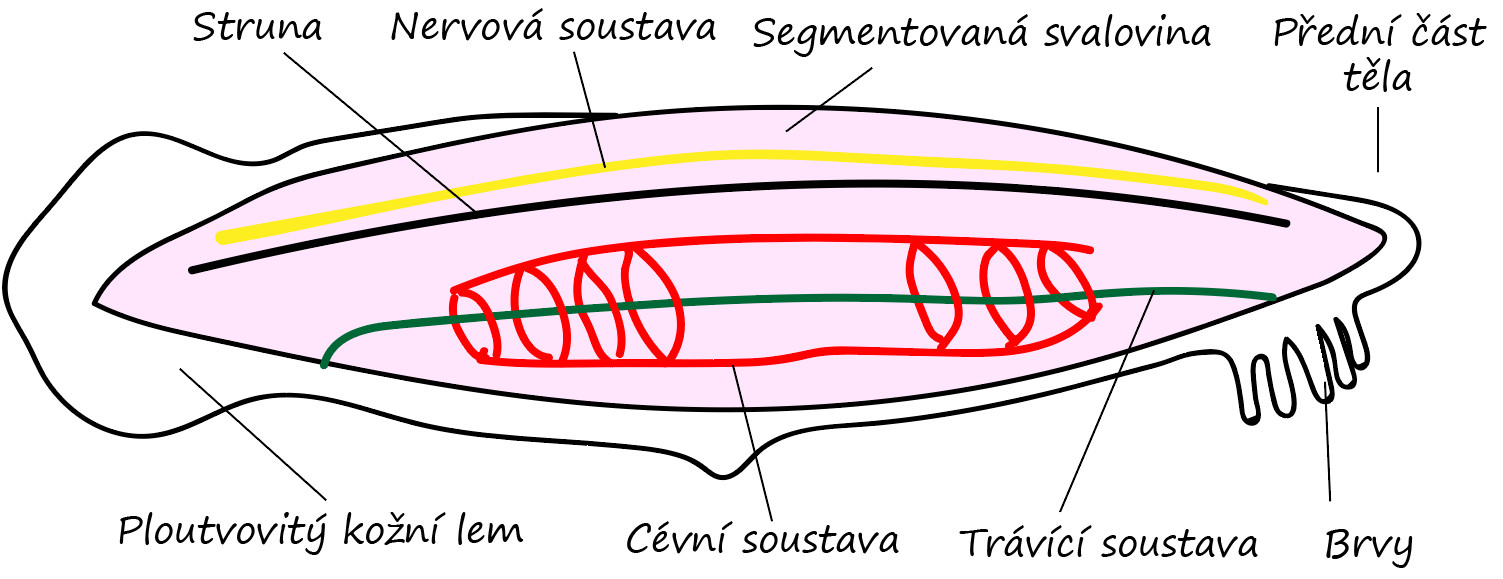
\includegraphics[width=1\textwidth]{pictures/kopinatec.png}

\section{Podkmen: Obratlovci \textit{(Vertebrata)}}
\subsection{Základní charakteristika obratlovců}
Živočichové $>$ Triblastica $>$ Druhoústí $>$ Strunatci $>$ Obratlovci
\begin{itemize}
\item nejpočetnější podkmen strunatců
\item \textbf{aktivně pohybliví}, bilaterálně souměrní
	\begin{itemize}
	\item příčně pruhovaná, hladká, srdeční svalovina
	\end{itemize}
\item mimořádně výkonná NS a smyslové orgány
\item tělo členěno na \textbf{hlavu, trup a ocas}
\item \textbf{pokožka} vždy \textbf{vícevrstevná}, produkuje různé deriváty (šupiny, peří, srst, \ldots)
\item struna hřbetní potlačena u dospělých jedinců a nahrazena vnitřní koštěnou kostrou s malým podílem chrupavek
\item končetiny mají jednotný stavební plán, mají koštěnou vnitřní stavbu
\end{itemize}

\subsection{Systém}
\begin{tabular}{|c|c|c|c|c|c|c|c|}
\hline
Třídy&kruhoústí&paryby&ryby&obojživelníci&plazi&ptáci&savci		\\ \hline
Přítomnost čelistí&bezčelistnatci& \multicolumn{5}{c}{čelistnatci} &		\\ \hline
Prostředí, kde žijí & \multicolumn{2}{c}{ploutvovci (Pisces)} && \multicolumn{3}{c}{čtyřnožci (Tetrapoda)} &\\ \hline
Prostředí vývoje vajec & \multicolumn{3}{c}{bezblanní (Anamnia)} && \multicolumn{2}{c}{blanatí(Amniota)} &		\\ \hline
\makecell{Schopnost udržovat \\ stálou tělesnou teplotu}	& \multicolumn{4}{c}{ektotermní} && \multicolumn{1}{c}{endotermní} &	\\ \hline
\end{tabular}

\paragraph{Přítomnost čelistí}
\begin{itemize}
\item čelisti vytvořeny z prvního páru žaber
\item bezčelistnatí mají 7 párů žaber
\end{itemize}

\paragraph{Prostředí}
\begin{itemize}
\item podobnosti ve stavbě ploutví a nohou
\end{itemize}

\paragraph{Prostředí vývoje vajec}
\begin{itemize}
\item bezblanní(\textit{Anamnia}) se rozmnožují ve vodě
\item blanatí (\textit{Amniota}) má vnitřní vodní prostředí \ra mohou se rozmnožovat na souši
\end{itemize}

\paragraph{Udržování teploty}
\begin{itemize}
\item studenokrevní (ektotermní)
\item teplokrevní (endotermní) -- velká spotřeba energie
\end{itemize}

\section{Nadtřída: Bezčelistnatci \textit{(Agnatha)}}
\begin{itemize}
\item 7 párů žaber
\item hadovitý tvar těla
\item produkce slizu -- snižuje riziko uchopení predátorem
\end{itemize}

\subsection{Třída: Kruhoústí \textit{(Cyclostomata)}}
\subsubsection{Podtřída: Sliznatky (\textit{Myxinoidea})}
\begin{itemize}
\item obývají mořské dno
\item destruenti -- vyžírají orgány z mrtvých / velmi zraněných ryb
\end{itemize}

\subsubsection{Podtřída: Mihule (\textit{Petromyzontida})}
\begin{itemize}
\item larva \textbf{minoha}
	\begin{itemize}
	\item pilovitý ústní disk \ra prořezávání ryb
	\end{itemize}
\item regresní vývoj (dospělec má zakrnělou trávící soustavu -> žije jen ze zásob a pak umře)
\end{itemize}

\paragraph{Mihule potoční, Mihule mořská}
\begin{itemize}
\item kriticky ohrožená
\end{itemize}


\section{Nadtřída: Čelistnatci \textit{(Gnathostomata)}}
\subsection{Třída: Paryby \textit{(Chondrichthyes)}}
\begin{itemize}
\item jednostranně orientované šupiny -- brání přisávání živočichů
\item vodní, převážně mořští
\item první objevení na konci prvohor a hlavní rozšíření v druhohorách
\end{itemize}

\paragraph{Tělo}
\begin{itemize}
\item velký rypec na přední straně
\item \textbf{Lorenziho ampule} (orgán) -- vnímá elektrické signály nervových soustav jiných živočichů
\end{itemize}

\subsubsection{Skupina: Chiméry \textit{(Holocephali)}}
\begin{itemize}
\item bizarně vypadající paryby
\item nepravá skřele -- krytka žáber
\end{itemize}

\subsubsection{Skupina: Příčnoústí \textit{(Elasmobranchii)}}
\begin{itemize}
\item torpédovitý tvar
\item dlouhý rypec, ústa na spodní straně hlavy
\item struna zachována po celý život
\item první pár žaber přeměněn v čelisti, druhý pár v jazylku
\item \textbf{plakoidní šupiny}
\begin{itemize}
\item jediný výskyt kostní tkáně (tvořeny -- dentinem a emailem), zakotveny ve škáře
\end{itemize}
\end{itemize}

\paragraph{Kostra}
\begin{itemize}
\item široká lebka s pouzdry smyslových orgánů
\end{itemize}

\paragraph{Ploutve}\mbox{} \\ \mbox{} \\
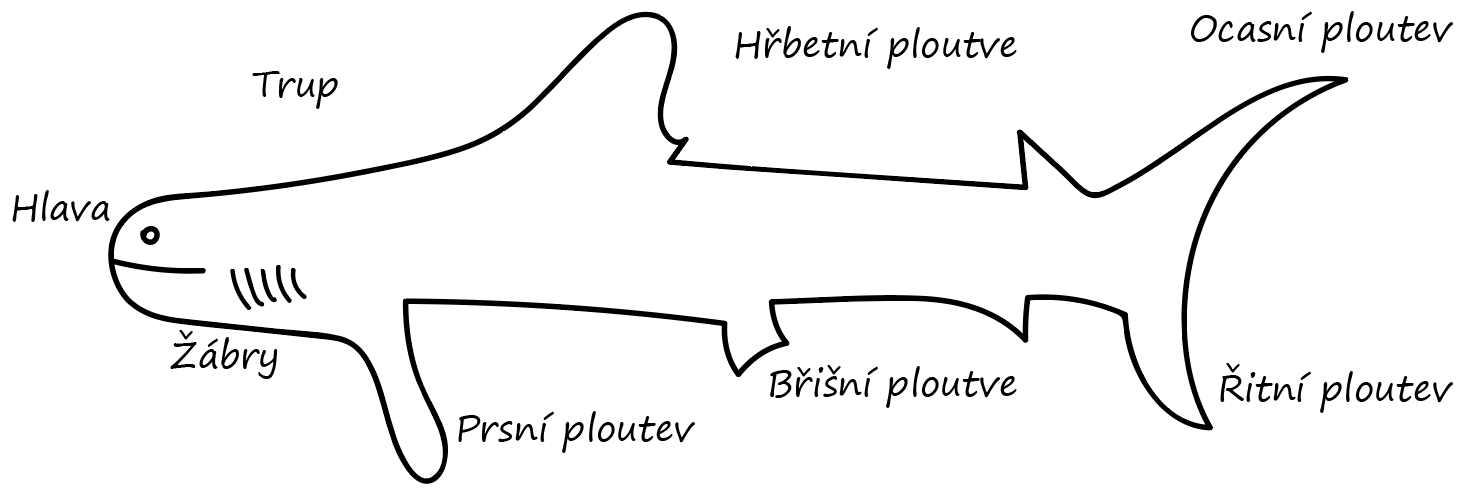
\includegraphics[width=\textwidth]{pictures/ploutve.png}


\paragraph{Nervová soustava}
\begin{itemize}
\item protáhlý mozek (už ne jen zauzlina)
	\begin{itemize}
	\item vyvinutý mozeček -- zodpovědný za koordinované pohyby
	\item čelní lalok -- čich
	\end{itemize}
\end{itemize}

\paragraph{Trávící soustava}
\begin{itemize}
\item ústa, zuby, hltan, jícen, žaludek, střevo
\item obrovská játra (10 - 20\% hmotnosti jedince) se žlučníkem 
\item hydrostatický orgán -- regulace hloubky ponoru
\item hypertonické prostředí \ra orgán na vylučování soli
\end{itemize}

\paragraph{Dýchací soustava} -- 2 páry žaber přeměněné na čelisti a jazylku, 5 párů zbylo

\paragraph{Cévní soustava} -- uzavřená, 1 předsíň, 1 komora, okysličení krve v žábrách

\paragraph{Rozmnožovací soustava}
\begin{itemize}
\item vnitřní oplození pomocí prsních ploutví
\item může se objevit živorodost (není placenta, ale žloutkový vak)
\item prenatální kanibalismus -- mláďata se mohou před narozením navzájem sníst
\end{itemize}


\paragraph{Ekologie}
\begin{itemize}
\item původně mořští, cca 30 sladkovodních druhů (15 smíšených)
\item podle druhu potravy dělíme na: lovce, plakntonofágy, bentofágy (rytí ve dně)
\end{itemize}

\paragraph{Chování} -- málo dlouhé, loví se k jídlu

\paragraph{Zástupci}
\begin{itemize}
\item \textbf{Žralok obrovský} -- planktonofágní
\item \textbf{Žralok bílý} -- 7m, 3.5t, nebezpečný pro člověka (živí se tvory u hladiny)
\item \textbf{Kladivoun obecný}
	\begin{itemize}
	\item oci na koncích hlavy
	\item velké množství Lorenziho ampulí na hlavě (elektrosensor)
	\end{itemize}
\item \textbf{Piloun mnohozubý} -- pentofág
\item \textbf{Trnucha obecná} -- u ocasu trn s jedovou žlázou, evropská pobřeží
\item \textbf{Manta atlanská} -- 9m 
\end{itemize}




\section{Třída: Ryby \textit{(Osteichthyes)}}
\begin{itemize}
\item dle reálného členění by pod ryby spadal i člověk (pod plazy ptáci) \ra třída ryby reálně neexistuje
\end{itemize}

\paragraph{Kostra a svaly}
\begin{itemize}
\item podélné boční svalstvo
\item kost poprvé převažuje nad chrupavkou
\item \textbf{skřele} -- kryjí žaberní dutiny
\end{itemize}

\paragraph{Morfologie}
\begin{itemize}
\item hydrodynamický tvar
\item kůže obsahuje slizotvorné žlázy, pigmenty, šupiny -- dělíme:
	\begin{itemize}
	\item ganoidní  -- primitivní ryby\ra bichiři, chrupavčití
	\item cykloidní -- snadno se oddělávají \ra máloostní, lososovití
	\item ktenoidní -- drsná, ostrá pokožka -- zoubky, špatně se oddělávají \ra ostnoploutví
	\end{itemize}
\end{itemize}

\paragraph{Ploutve}
\begin{itemize}
\item celistvá ocasní ploutev dělení na: hetrocerkní, difycerkní, homocerkní
\item prsní ploutve navázané na lebku  \ra pletenec (možnost vývoje chození po čtyřech)
\end{itemize}

\includegraphics[width=0.65\textwidth]{pictures/ocasni_ploutve.png}

\paragraph{Nervová soustava}
\begin{itemize}
\item značně potlačený čich oproti parybám
\item výrazně zlepšený zrak, chybí oční víčka, čočka se nedeformuje ale posouvá
\item mozek s vyvinutými laloky a mozečkem
\item postranní čára -- proudový orgán
	\begin{itemize}
	\item voda proniká kanálky do receptorů 
	\end{itemize}
\end{itemize}

\paragraph{Trávící soustava}
\begin{itemize}
\item trubicovitá
\item tři typy úst: 
	\begin{itemize}
	\item svrchní -- hmyz nad hladinou
	\item koncová -- dravci
	\item spodní -- ryjí v bahně, + vousy
	\end{itemize}
\end{itemize}

\paragraph{Dýchací soustava}
\begin{itemize}
\item 5. pár žaberních oblouků přeměněn na \textbf{požerákové zuby} (\ra zbývají 4)
\item žábry kryté skřelemi
\item přídatné dýchací orgány -- jsou schopné přijímat kyslík i hltanem, žaludkem a hydrostatickým orgánem
\end{itemize}

\paragraph{Cévní soustava}
\begin{itemize}
\item venózní srdce uložení na břišní straně těla
\item velké, oválné červené krvinky, mají jádro
\end{itemize}

\paragraph{D.ú.: Která ryba řeší jaký problém se solí?}
\begin{itemize}
\item sladkovodní ryba se musí zbavovat vody (nezahuštěná moč)
\item sladnovodní ryba se musí zbavovat soli (zahuštěná moč)
\item migrující ryby to maj blbý
\end{itemize}

\paragraph{Zástupci}
\begin{itemize}
\item ďas mořský
\item okoun říční -- vidí dobře ve špinavé vodě (velké oči \ra okoun)
\item kapr
\item sumec velký -- čistí dno (bacha ať vám nesní děcko!)
\item vranka -- v horních tocích řek \ra úzké tělo proti proudu, drápky na prsních ploutvích
\end{itemize}


\paragraph{Rozmnožování}
\begin{itemize}
\item většinou gonochoristé, vnější oplození (vejcorodí)
\item živorodí (3\%) využívají řitní ploutev jako kopulační orgán
\item mlíčňák -- samec
\item jikernačka -- samice
\item tření -- rozmnožování
\item trdliště -- místo tření
\end{itemize}

\paragraph{Ekologie -- potravní adaptace}
\begin{itemize}
\item všežravé (\textit{omnivorní}) -- živí se drobnými druhy živočichů a občas i rostlinnou potravou
\item bentofágní -- ryje do dna (červy, měkkýši, larvy)
\item madreporofágní (durofágní) -- požírají živočichy s tvrdými skořápkami
\item planktonofágní -- živí se planktonem
\item dravé ryby -- lový jiné ryby
\item fitofágní
\end{itemize}

\paragraph{Rybí pásma}
\begin{itemize}
\item \textbf{pstruhovité} -- čisté, hodně okysličené, studené vody
\item \textbf{lipanovité} -- podhorské potoky a říčky, teplejší ale čistá
\item \textbf{parmové} -- střední úseky řek, široké, hluboké, rychlé
\item \textbf{cejnové} -- nížinné, i stojaté, mnoho sedimentu, málo kyslíku, teplé vody
\end{itemize}

\paragraph{Další ekologické skupiny}
\begin{itemize}
\item \textbf{pelagické} -- na volném moři v různých hloubkách (sledi, sardinky)
\item \textbf{litorální} -- v mělčinách při pobřeží
\item \textbf{bentické} -- obývající mořské dno
\item \textbf{brakické} -- v ústí řek do moře
\item \textbf{tažné}
	\begin{itemize}
	\item katadromní -- za třením z řek do moře (úhoř)
	\item anadromní -- za třením z moře do řek (losos, jeseter)
	\end{itemize}
\end{itemize}


\subsection{Podtřída: Dvojdyšní (\textit{Dipnoa})}
\begin{itemize}
\item dvojdyšní = mají jak žábry, tak plicní vaky
\item velké protáhlé tělo
\item Bahník se v období sucha zahrabe do bahna a hybernuje
\end{itemize}

\subsection{Podtřída: Lalokoploutví (\textit{Crossopterygii)}}
\begin{itemize}
\item téměř vyhynulí
\item největší rozšíření v devonu
\item považují se za předky suchozemských živočichů
\item velké (několik cm) kožovité vejce
\end{itemize}

\subsection{Podtřída: Paprskoploutví (\textit{Actiniptererygii})}
\begin{itemize}
\item 99\% ryb
\end{itemize}

\subsubsection{Nadřád: Chrupavčití (Chondrostei)}
\begin{itemize}
\item chrupavčitá kostka
\item hlava je protažená v rypec (rostrum) s hmatovými výrůstky
\item heterocerkní ocasní ploutev
\item jikry se používají jako kaviár
\end{itemize}

\paragraph{Zástupci}
\begin{itemize}
\item jeseter velký, malý
\item viza velká -- až 8m, kvalitní kaviár, velmi ohrožená
\end{itemize}

\subsubsection{Nadřád: Mnohokostnatí (\textit{Neopterygii})}
\begin{itemize}
\item velmi stará skupina ryb
\item dificerkní ploutev
\end{itemize}

\paragraph{Řád: Kostlýni}
\paragraph{Řád: Kaprouni}

\subsubsection{Nadřád: Kostnatí (\textit{Teleostei})}
\begin{itemize}
\item 99\% ryb
\item osifikovaná (zkostnatělá) kostra
\item homocerkní ocasní ploutve
\end{itemize}

\paragraph{Zástupci}
\begin{itemize}
\item pstruh duhový, stříbrný
\item lipan podhorní (dravý)
\item losos
\item štika (dravá, torpédo)
\item karas
\item kapr obecný
\item amur bílý (z Ruska)
\item cejn velký
\item lín obecný
\item candát obecný
\item jeseter velký
\item makrela obecná
\item sardinka obecná
\item sleď obecný
\item treska obecná
\end{itemize}

\newpage
\section{Třída: Obojživelníci \textit{(Amphibia)}}
\begin{itemize}
\item přechod mezi vodními a suchozemskými obratlovci (rozmnožování ve vodě)
\item nejstarší známí -- \textbf{krytolebci}
\item vznik z lalokoploutvých ryb
\item dosahovali až 1m
\item dnes cca 3000 druhů
\end{itemize}

\paragraph{Dýchací soustava}
\begin{itemize}
\item larva -- vnější keříčkovité žábra
\item dospělci -- plíce
\item 5. žeberní oblouk přeměněn na jazylku
\end{itemize}

\paragraph{Kostra}
\begin{itemize}
\item zkostnatělá (ostnifikovaná)
\item lebka je kloubně spojena s páteří \ra otáčení hlavy
\item žáby -- hrudní kost (chybí koš)
\item 4--5 prsté končetiny s plovacími blánami
\item \textbf{urostyl} -- srůst obratlů v bederní části v jednotnou kost usnadňující skákání
\end{itemize}

\paragraph{Kůže}
\begin{itemize}
\item lysá, četné slizové, případně jedovaté žlázy
\item pigmentové buňky -- chromatofory
\item prokrvená -- kožní dýchání
\item svlékání a požírání
\end{itemize}

\paragraph{Vylučovací soustava}
\begin{itemize}
\item párové prvoledviny
\item močový měchýř
\item kloaka
\end{itemize}

\paragraph{Cévní soustava}
\begin{itemize}
\item 
\end{itemize}

\paragraph{Nervová soustava}
\begin{itemize}
\item trubicovitá
\item nejvýznamější částí mozku je střední mozek
\item malý mozeček
\item střední ucho u dospělců
\end{itemize}

\paragraph{Smysly}
\begin{itemize}
\item dobře vivinuté oči, tři víčka
\item parietální orgán (temeno hlavy) -- světlo x tma
\item čich v nosní dutině -- poprvé Jacobsonův orgán
\item proudový orgán u larev
\item sluch -- bubínek na povrchu hlavy, sluchová kůstka (columella), vnitřní ucho, Eustachova trubice
\end{itemize}

\subsection{Podtřída: Beznozí \textit{(Apoda)}}
\begin{itemize}
\item starobylí
\item tropy
\end{itemize}

\paragraph{Zástupci}
\begin{itemize}
\item Červor vodní
\end{itemize}

\subsection{Podtřída: Ocasatí \textit{(Caudata)}}
\begin{itemize}
\item ještěrkovitý tvar těla
\item dva páry končetin
\item redukovaný sluch, drobné zuby, velká schopnost regenerace
\item vnitřní oplození
\end{itemize}

\subsection{Podtřída: Bezocasí \textit{(Anurar)}}
\begin{itemize}
\item krátké zavalité tělo bez ocasu
\item zadní končetiny mnohem delší
\item mezi prsty zadních končetin plovací blána
\item jazyk -- může být vymrštěn dalseko a slouží k lovu kořisti
\item většina žab přizpůsobena k suchozemskému životu
\item oční víčka
\item mnohé žáby pečují o svá vajíčka
\item amplexus -- způsob chycení samičky při páření
\end{itemize}

\paragraph{Kuňka}
\begin{itemize}
\item kuní efekt
\end{itemize}

\paragraph{Ropucha}
\begin{itemize}
\item klade vajíčka do provazu
\end{itemize}


\paragraph{Skokani}
\begin{itemize}
\item štíhlé žáby
\item nejhojnější je skokan hnědý
\item mimo rozmnožování jsou ve stinných lesích
\item klade vajíčka do chuchvalce
\end{itemize}

\paragraph{Blatnice}
\begin{itemize}
\item svislé zorničky oka
\item noční žába
\item vyhrabává si nory
\item obrovští pulci (až 20cm)
\end{itemize}

\paragraph{Rosnička}
\begin{itemize}
\item žijí na stromech a keřích
\item pohybuje se dobře na hladkých plochách
\item vyluzuje různé zvuky podle změny tlaku
\end{itemize}

\paragraph{Pralesnička strašná}
\begin{itemize}
\item má 1mg jedu, který stačí k zabití 10--20 lidí nebo 2 samce slona afrického
\end{itemize}

\paragraph{Veleskokan africký}

\paragraph{Hrabatka drsná}


\paragraph{Opakování}
\begin{enumerate}
\item Kůže obojživelníků slouží k \ldots
\item Obojživelníci patří mezi teplokrevné živočichy: ANO $\times$ NE
\item Pulci dýchají \ldots
\item Dospělci dýchají \ldots
\item Jak od sebe rozeznáš pulce čolka a žáby?
\item Jaké druhy žab u nás můžeš najít?
\end{enumerate}

\section{Třída: Plazy \textit{(Reptilia)}}
\paragraph{Přechod na souš}
\begin{itemize}
\item k přechodu vodních obratlovců na souš došlo na konci devonu -- nejprimitivnější obojživelníci (před cca 350 mil. let)
	\begin{itemize}
	\item na souši je více potravy, není tam žádná konkurence
	\item vysychají mělké sladké vody
	\item na souši je větší teplo (studenokrevní)
	\end{itemize}
\end{itemize}

\paragraph{Adaptace při přechodu na souš}
\begin{itemize}
\item \textbf{pokryv těla} -- silná kůže se zrohovatělou pokožkou, která vytváří rohovité šupiny (ještěři a hadi vrstvu šupin při růstu svlékají), výborně izoluje proti ztrátám vody, kožní žlázy prakticky chybí
\item \textbf{vytvoření dýchacích orgánů} -- znemožněné kožní dýchání \ra vznik plyc, redukce žaber
\item \textbf{změna cévní soustavy} -- vytvoření dvou oběhů, malý plicní a vělký tělní, dvě síně, dvě komory
\item přeměna ploutví v končetiny
\item ostifikace kostry -- nese váhu celého organismu
\item pohyblivé spojení lebky s páteří a vznik krku
\item připojíení pletence horní i dolní končetiny k páteři
\item vytvoření hrudního koše, který chrání měkké vnitřní orgány
	\begin{itemize}
	\item musí být pohyblivý kvůli dýchání
	\end{itemize}
\end{itemize}

\paragraph{Amniota}
\begin{itemize}
\item plazy již patří mezi blanaté \ra mohou se plně odpoutat od vodního prostředí
\item amnion, allantois, chorion -- tři zárodečné blány
\item žloutek, bílek, skořápka
\end{itemize}

\paragraph{Trávící soustava}
\begin{itemize}
\item ústní dutina, dlouhý vysunovatelný jazyk
\item pomalé, efektivní trávení
\item kloaka
\end{itemize}

\paragraph{Dýchací soustava}
\begin{itemize}
\item plícemi, pokožka nepropustná
\item chybí hlasové ústrojí
\item nejvyvinutější srdce u krokodýlů -- čtyřdílné
\end{itemize}

\paragraph{Vylučovací soustava}
\begin{itemize}
\item párové ledviny, močový měchýř u želv a ještěrů
\item urikotelní -- vylučují dusík v kyselině močové \ra kašovitá moč
\end{itemize}

\paragraph{Nervová soustava}
\begin{itemize}
\item plazi mají nejvyvinutější koncový mozek a mozeček
\item 12 párů mozkových nervů
\end{itemize}

\paragraph{Smysly}
\begin{itemize}
\item Jacobsonův orgán -- umožňuje vnímat pach látek rozpuštěných ve slinách
\item dokonalý zrak
\item schopnost akomodace -- pohyb oka v prostředí
\item tři víčka -- mžurka
\end{itemize}

\paragraph{Rozmnožování}
\begin{itemize}
\item párové gonády
\item častý sexuální dimorfismus
\item pohlavní pomocí kloaky
\item vejcorodí
\end{itemize}

\subsection{Řád: Krokodýli}
\begin{itemize}
\item nejvyspělejší
\item kryté, těžko zranitelné tělo
\item plochá hlava s protaženou tlapou
\item oči shora -- pozorují pod i nad hladinu
\item živí se dravě a sami jsou často loveni člověkem pro kůži
\end{itemize}

\paragraph{Krokodýl $\times$ aligátor}
\begin{itemize}
\item krokodíl -- delší hlava, protáhlejší tělo, čtvrtý zub venku
\item aligátor -- kratší hlava, mohutnější tělo schovaný čtvrý zub
\end{itemize}

\paragraph{Zástupci}
\begin{itemize}
\item aligátor americký
\item krokodýl mořský -- největší zástupce (8m, 2t), žije v brakické vodě
\item gaviál indický -- tenká, protáhlá čelist, živí lovem ryb
\end{itemize}

\subsection{Řád: Šupinatí}
\begin{itemize}
\item nejpočetnější
\end{itemize}

\subsubsection{Podřád: Ještěři}
\begin{itemize}
\item \textbf{autotomie} -- schopnost ztratit končetinu (ocas)
\item vyvinuté končetiny, pohyblivá víčka
\end{itemize}

\paragraph{Zástupci}
\begin{itemize}
\item ještěrka živorodá, zelená, skalní a obecná
\item chameleon -- umí přivřít víčko, barvoměna, nezávislý pohyb
\item bazilišek zelený -- není had!, dlouhý ocas, rotační kyčle \ra rychle běhá, klidně i po vodě
\item varan komodský
\end{itemize}

\subsubsection{Podřád: Hadi}
\begin{itemize}
\item plazi s protáhlým tělem a redukovanými končetinami
\item jedovaté zuby, rozeklaný jazyk
\item redukovaná levá plíce
\item srostlá a průhledná oční víčka, v celku se svléká kůže
\end{itemize}

\paragraph{Užovka $\times$ zmije}
\begin{itemize}
\item zmije má svislý tvar zornice -- "zlý pohled"
\item užovka má větší šupiny
\end{itemize}

\paragraph{Zástupci}
\begin{itemize}
\item užovka obojková -- loví ryby
\item užovka podplamatá
\item užovka stromová -- náš nejdelší had, loví myši
\item zmije obecná
\item kobra královská -- odolná vůči svému jedu, loví mangusty (jsou též odolní)
\end{itemize}

\subsection{Řád: Želvy}
\begin{itemize}
\item staré, 10cm--2m
\item silné krátké končetiny
\item dělíme na suchozemské a vodní
\end{itemize}

\paragraph{Zástupci}
\begin{itemize}
\item želva bahenní -- malá populace
\item želva nádherná -- červená skvrna za okem, často chovaná
\item dlouhokrčka australská -- neumí zatahovat krk do krunýře
\item kajmanka supí -- masožravá, trnitý krunýř, může ukousnout nohu
\item želva sloní -- Galapágy, využívány jako "živé konzervy"
\item želva zelenavá -- jihovýchodní Evropa , 
\item kareta obrovská -- mořská, zachytávají se za sítě \ra udusí se
\item kožatka velká -- mořská, měkčí krunýř, než kareta
\end{itemize}

\paragraph{Krunýř}
\begin{itemize}
\item 
\end{itemize}


\subsection{Řád: Haterie}
\paragraph{Hatérie novozélandská}
\begin{itemize}
\item "živé zkameněliny"
\item světločivné temenní oko na zádech
\end{itemize}


\section{Třída: Ptáci \textit{(Aves)}}
\begin{itemize}
\item zadržují vodu -- pijí zakloněním hlavy, neumí polykat
\item vidličková kost -- pružina pro křídla
\item teplokrevní
\item důležitý zrak -- ostří posouváním čočky dopředu dozadu
\item vytvořen běhák
\item čtyřdílné srdce
\item homiotermie
\item zehříání vajíček a obvykle i péče o potomstvo
\end{itemize}

\paragraph{Modifikace k letu}
\begin{itemize}
\item křídla, peří, 
\item duté kosti (chybí kostní dřeň), srůsty na kostře, strenální hřeben (hrudní kost)
\item rozvoj létacíhc svalů
\item vzdušné vaky
\item častá defekace a hustá moč

\end{itemize}

\paragraph{Peří}
\begin{itemize}
\item typy
	\begin{itemize}
	\item letky -- velká plocha
	\item rýdovací -- kormidlo
	\item krycí -- drží teplo
	\item prachové peří -- 
	\end{itemize}
\end{itemize}

\paragraph{Kostra}
\begin{itemize}
\item velká oční koule v lebce
\item vyvinutý atlas a axis \ra umožněn rotační pohyb lebky
\item sternální hřeben na kterém jsou upnuty prsní svaly
\item na noze vratiprst
\item modifikace končetin -- spáry, plováky (blána), brodivá
\end{itemize}

\paragraph{Smysly}
\begin{itemize}
\item dominantní zrak
	\begin{itemize}
	\item pecten -- žlutá skvrna u dravců
	\item proměnlivý tvar oka, čočka se posouvá
	\end{itemize}
\item špatný čich, lepší u mrchožroutů
\end{itemize}

\paragraph{Rozmnožování}
\begin{itemize}
\item kloaka
\item běžci mají vyvinutý penis
\end{itemize}

\paragraph{•}
\begin{itemize}
\item vývržky nestrávené potravy
\end{itemize}

\paragraph{Dýchací soustava}
\begin{itemize}
\item vzduch se ukládá do výběžků
\item prochází přes plíce při vdechu i výdechu
\item syrinx -- zvukové ústrojí (na místě rozdvojení průdušnice)
\end{itemize}

\paragraph{Vylučovací soustava}
\begin{itemize}
\item ledviny
\item urikotelní moč -- 
\end{itemize}

\paragraph{Etologie}
\begin{itemize}
\item nidifugní -- nekrmivá mláďata
\item nedikolní -- krmí mláďata
\end{itemize}

\end{document}